\chapter{相关研究综述}
\label{cha:review}

\section{故障预测与健康管理}
\label{sec:review-phm}

% 如图\ref{fig:phm-maintenance}所示故障维修体制发展至今可划分为三个时期,即事后维修(又称无计划维修)、计划性维修和视情维修\cite{jardine2006review}。早期工业系统复杂性和安全性要求较低,采用事后维修即可满足需求。随着安全性需求不断提升,维修体制逐渐向计划维修过渡,即对系统进行定期检查、保养和维修以延长系统寿命、降低系统故障风险。社会工业科技不断进步,系统集成度越来越高、复杂性不断增加,劳动密集型的计划维修体制费时费力、效率低下,维修成本不断攀升以至于已经成为很多工业公司的主要支出\cite{peng2010current}。在此背景下,维修技术逐渐过渡到高效的视情维修\cite{jardine2006review,peng2010current}。视情维修主要由数据获取、数据处理和维修决策三个步骤组成,基于获取的数据以数据处理为手段挖掘潜在价值实现系统故障诊断和预测,进而作出是否采取维修行为的决策。视情维修很大程度避免了计划维修中非必要的维修投入。
% \begin{figure}[H]{}
% \centering
% 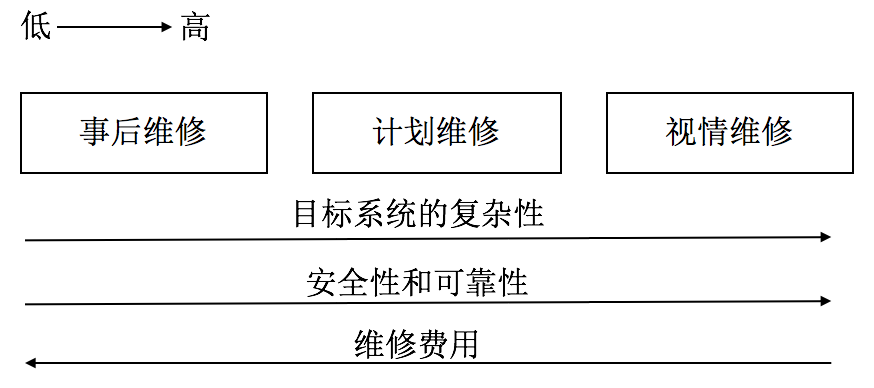
\includegraphics[scale=0.5]{figures/phm-maintenance.png}
% \caption{维修体制进化路线}
% \label{fig:phm-maintenance}
% \end{figure}
故障预测与健康管理(PHM)技术是实现视情维修的有效手段,是利用大数据技术和机器学习技术,把失效机制、寿命预测和全生命周期管理整合在一起进行统筹化的系统工程\cite{lee2014prognostics}。本文将PHM系统工程的主要内容归纳为图\ref{fig:phm-framework}。目前在国外尤其是美国 PHM 系统已投入应用,比如美军的 F-35 战斗机已全面部署 PHM 系统,取消计划性检修,大大降低了系统维修开销\cite{brown2007prognostics}。PHM 技术的有效性得到验证后倍受关注,正迅速覆盖除军事以外的民用技术领域,比如 民航、交通、船舶、制造业等领域。相比之下,国内的PHM技术正处于起步阶段,研究主要基于航空航天、船舶等高技术复杂装备展开\cite{彭宇2010故障预测与健康管理技术综述},大部分复杂工业系统仍沿用计划维修体制。因此,如何利用 PHM 技术实现中国维修体制的转型仍是一个亟待解决的问题。
\begin{figure}[H]
\centering
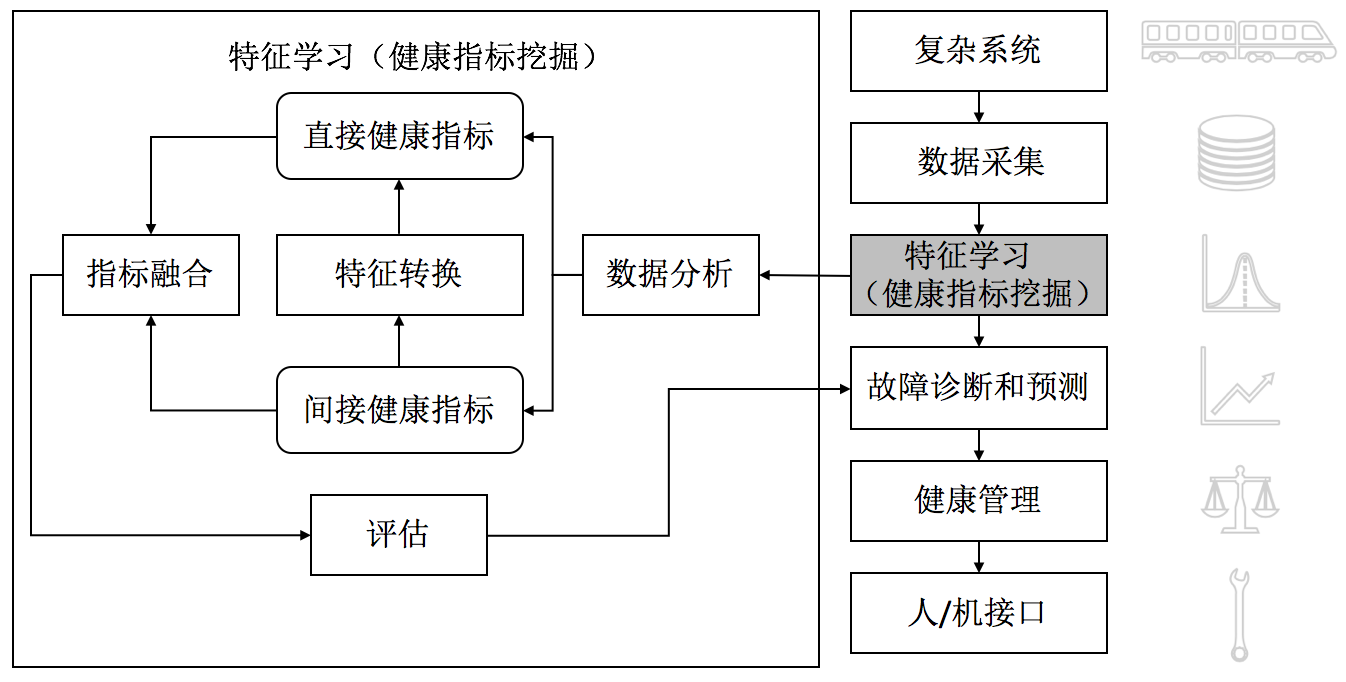
\includegraphics[scale=0.5]{figures/phm-framework.png}
\caption{PHM 系统工程}
\label{fig:phm-framework}
\end{figure}
故障预测是 PHM 的核心要义,其划分大同小异,比如Si 等人将故障预测方法分为四类,即基于实验的、数据驱动的、基于物理模型的和混合的故障预测方法\cite{si2011remaining};Lee 等人划分为三类,即基于模型的、数据驱动的和混合的故障预测方法\cite{lee2014prognostics};彭宇等人分为三类,即基于模型的、数据驱动的和基于统计可靠性的故障预测方法\cite{彭宇2010故障预测与健康管理技术综述};Pecht 等人分为两类,即基于模型的和数据驱动的故障预测方法\cite{pecht2010prognostics}。为便于讨论和研究,本文统一将故障预测方法划分为以下两类:

1. 基于模型的故障预测方法:基于模型的故障预测方法依赖精确的物理模型和专家知识建模,通过对比观测数据与内置精确模型仿真数据的差异来发现和预测故障。比如Byington 等人采用基于模型的故障预测方法实现飞机控制部件的故障预测,需要配置精确的物理模型实现参数估计\cite{byington2004model}。由于有精确的物理模型为基础,基于模型的故障预测方法预测精度最高。然而在全球化趋势下获得清晰准确的机理知识困难甚至不可能。因此,基于模型的故障预测方法应用领域较窄,局限于系统机理透明并且对精度要求很高的领域,如军用装备领域。

2. 数据驱动的故障预测方法:数据驱动的故障预测方法采用数据挖掘和机器学习技术,从历史运行数据中提取系统健康指标,并实现故障诊断和预测。比如获得PHM-2008竞赛冠军的 Wang 等人\cite{wang2008similarity},首先分析历史数据找到反应系统性能的关键信号,然后基于关键信号采用线性回归方法构建系统健康指标,最后使用基于相似性的分类方法实现系统剩余寿命预测。数据驱动的故障预测方法预测不依赖准确的机理知识,具有良好的灵活性便于实际应用,然而现有方法大多针对任务直接建模,缺乏对系统机理的认识。

工业大数据技术的成熟使数据驱动的故障预测方法倍受青睐\cite{tsui2015prognostics,si2011remaining},有少部分学者还提出混合模型的概念尝试融这两类模型的优点来提升故障预精度\cite{pecht2010prognostics}。针对工业系统采集的数据可分为事件数据和状态监测数据两类,其中状态监测数据是反应系统性能的最好依据,按数据类型可分为实值数据(比如温度、湿度等)、波形数据(比如震动信号、声学信号等)和多维数据(比如图片等)\cite{jardine2006review}。基于获取方式的不同,状态监测数据又可进一步分为直接状态监测数据和间接状态监测数据两类。由此衍生两大类数据驱动的故障预测方法,分别为基于直接状态监测数据的故障预测方法和基于非直接监测数据的故障预测方法\cite{si2011remaining}。

对于数据驱动的故障预测方法,如何有效的处理数据并挖掘具有反应系统状态变迁能力的特征或指标是关键,这一过程通常被称为健康指标(简称指标)提取\cite{pecht2010prognostics}。本文将健康指标提取过程以及其在PHM系统工程中所扮演的角色归纳为图\ref{fig:phm-framework}。系统健康指标可以分为以下两类\cite{zhou2011latent}:(a)直接指标,直接与系统失效机理相关,比如刹车片的厚度、齿轮裂纹深度等;(b)非直接指标,部分反应系统失效机理,如分析石油数据提取的特征。直接指标更难获取,但可以更精确反映系统的健康状态。非直接指标可通过特征转换的方式映射为直接指标\cite{si2011remaining,zhou2011latent}。


健康指标挖掘已得到广泛关注和研究。
Yan 等人,针对电梯门运动系统,通过逻辑斯蒂回归(Logistics Regression, LR)从多维数据中提取单维健康指标,并基于此利用ARMA实现剩余寿命预测\cite{yan2004prognostic}。
Wang 等人,针对涡扇发动机系统,以数据分析为基础从20多维传感器信号中找到与失效密切相关的6维关键信号,基于此通过线性回归构建单维系统健康指标,最后利用健康指标实现剩余寿命预测\cite{wang2008similarity}。
Patil 等人通过实验发现绝缘栅双极型晶体管(Insulated Gate Bipolar Transistors, IGBTs)的3个失效敏感信号可作为系统健康指标提取的基础\cite{patil2008failure}。
Zhou 等人指出状态空间模型提供了从非直接指标到直接指标的有效估计,针对现有状态空间模型高度依赖离散时间、离散状态、直线性和高斯性等假设的局限性,提出了一种不依赖以上假设的状态空间模型并采用基于蒙特卡罗的算法实现模型参数估计和剩余寿命预测,最后通过MATLAB进行数值仿真实验\cite{zhou2011latent}。
He 等人,针对齿轮震动信号,通过基于柯列斯分解的转换从多维相关震动信号中提取单维的反映系统健康状态的指标,并在此基础上利用滑动平均模型(Auto-Regressive and Moving Average Model, ARMA)实现剩余寿命预测\cite{he2012integrated}。
Liu 等人,针对锂离子电池系统,提出并设计了完整的健康指标提取框架,主要涉及数据转换、相关性分析、健康指标评估几个阶段\cite{liu2015health}。 

综上所述,健康指标挖掘是数据驱动的PHM方法的核心。然而现有的健康指标挖掘方法大多针对特定场景和系统部件进行建模设计,局限性较大,很难进行广泛应用。再者大多健康指标虽具有预测能力,但缺乏对系统底层机理的良好解释。针对以上问题,本文将结合物理系统动力学特性、复杂系统临界相变理论和机器学习技术,以数据驱动的方法为主要手段,同时充分利用可获取的先验知识,探索新方法从高维、高噪、时变的工业时间序列中挖掘反应系统状态变迁和运行机理的普适特征。另外本文将健康指标挖掘统称为{\heiti 特征学习}。

%\subsection{时间序列数据分析和特征学习方法}
\section{时间序列特征学习}
\label{sec:ts-representation-review}
% 时间序列的普遍性和重要性
% 时间序列的定义
% 时间序列分析的一般流程:数据采集 + 预处理 + 特征学习 + 任务
% 本文主要研究:预处理和特征学习,详细讨论
% 时间序列数据预处理方法:主要参考两本书
% 时间序列特征学习方法:按照现有分类进行概述

时间序列是普遍存在的重要数据类型,比如生态领域随时间变化的种群数量、金融领域随时间波动的经济指标、医疗领域随时间变化的生理指标、工业系统领域随时间变化的状态监测数据等都是时间序列\cite{aggarwal2015data}。一般的,时间序列数据由随时间变化的连续过程的采样点构成,是生态、金融、医疗和工业等领域的重要资源\cite{esling2012time,gaber2005mining}。

时间序列存在高维、高噪、时变等特点使其难以被开采利用,时间序列分析被认为是数据挖掘领域最具挑战的十个问题之一\cite{langkvist2014review}。对时间序列的开采过程通常可称为信号处理(Signal Process)\cite{rabiner1975theory}、时间序列分析(Time Series Analyais)\cite{bisgaard2011time}或时间序列挖掘(Time Series Mining)\cite{fu2011review}。从信号处理的角度,大多时间序列为电信号,比如震动信号、脑电波等,因此有很多时间序列开采方法都源于信号分析学,比如常见的傅立叶变换、正弦变换、余弦变换等信号转换方法,高通滤波、低通滤波、卡尔曼滤波等可以有效消除噪音影响的滤波方法。从时间序列分析的角度,大多方法倾向于分析时间序列的统计特性,比如时间序列的稳定性、自相关性等,应用场景多为时间序列预测。从时间序列挖掘的角度,更多强调利用数据挖掘和机器学习方法来对时间序列进行开采利用,应用场景除了传统的预测任务外还关注索引、分类、聚类、主题挖掘等任务\cite{fu2011review}。

本文统一采用{\heiti 时间序列挖掘}这一术语表示对时间序列数据的开采利用过程,关键流程归纳为图\ref{fig:tsm-framework},主要包含数据采集、特征学习及应用三个环节。其中,特征学习是数据得以有效利用的关键,一直是研究热点和难点\cite{langkvist2014review}。

\begin{figure}[H]
\centering
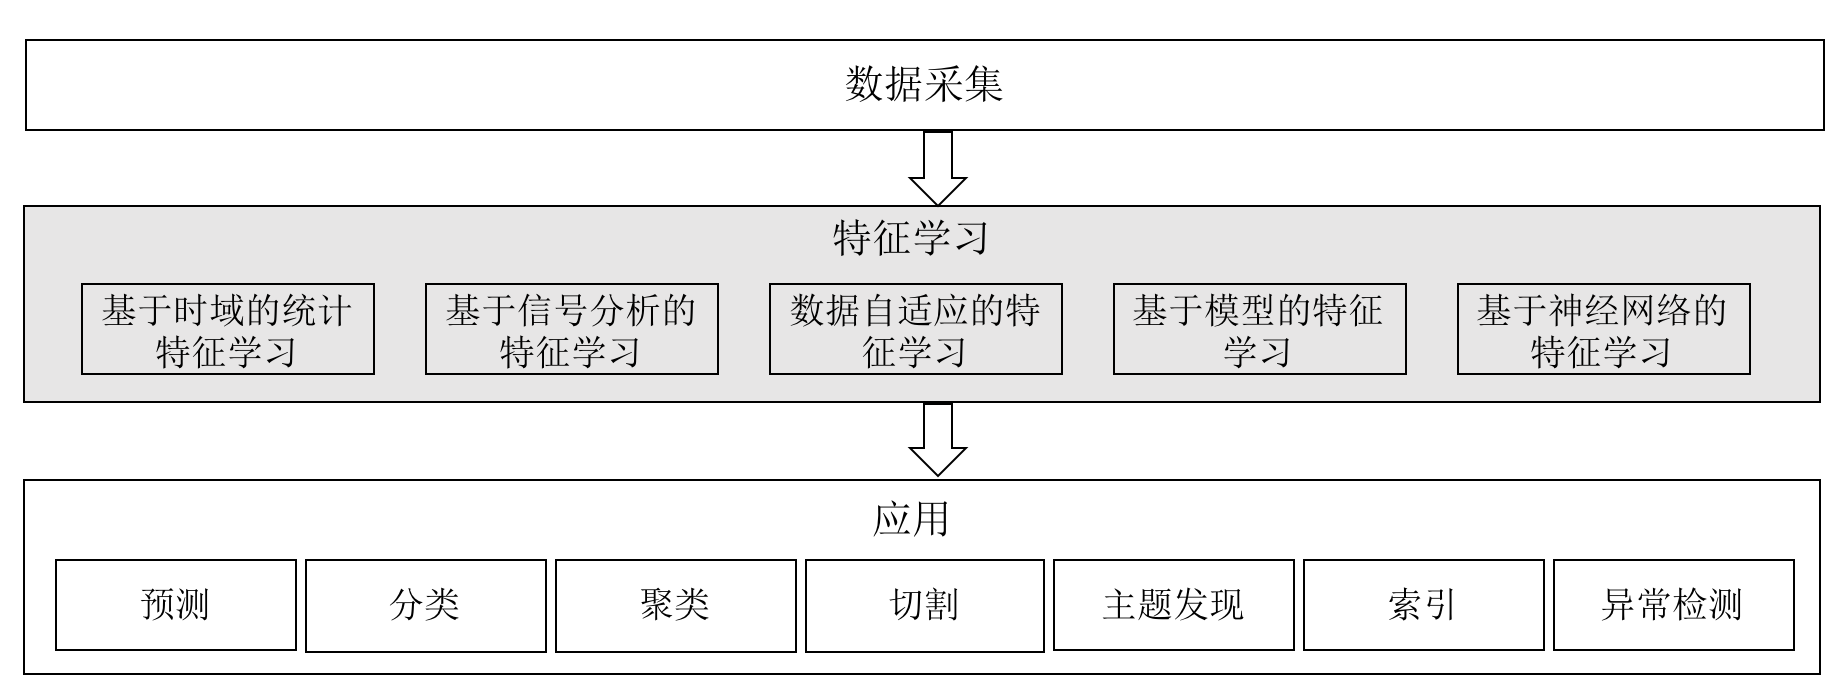
\includegraphics[scale=0.45]{figures/tsm-framework.png}
\caption{时间序列挖掘流程}
\label{fig:tsm-framework}
\end{figure}

\subsection{时间序列数据采集}

%“工业 4.0”的提出使工业数据得到有效的采集、传输和存储\cite{manyika2011big}。
工业数据主要通过传感器进行采集,为保证数据质量,此过程通常需要进行适当的预处理操作。

(1)数据集成

数据集成是指整合位于不同资源上的数据并为用户提供统一视图的过程\cite{lenzerini2002data}。在工业系统中,数据往往存放于不同数据库,再者不同系统、同一系统的不同部件的采样配置通常也有差异,因此数据集成是保证数据一致性的重要手段。
%最典型的不同采样率的时间序列数据需要进行时间对标以保证不同来源的观测值在时间上是一致的。

(2)重采样

采样率是时间序列数据采集过程的关键参数,并且因应用场景不同通常存在较大差异,因此不同来源的时间序列需进行时间对标以确保数据的一致性。此外过高的采样率容易导致冗余,而过低的采样率容易导致关键信息丢失。因此,在针对时间序列展开深入挖掘之前,通常先根据任务需求对数据进行上采样或下采样处理。上采样一般通过插值方法实现,下采样一般通过数据规约实现。处理信号数据时重采样往往会与滤波操作结合。更具体细节可参考Good 等人的著作\cite{good2006resampling}。
% 采样率是时间序列数据采集过程的关键参数。采样率在不同领域,或同一领域的不同场景通常存在较大差异,比如工业领域的传感数据通常以秒为单位间隔采样,而金融数据、天气数据、网络日志等数据通常以小时甚至以天或月份为采样间隔。因此不同来源的时间序列需进行时间对标以确保数据的一致性。此外,采样率高低直接影响数据的体量和蕴含信息的能力,过高采样容易导致冗余和大体量数据进而浪费资源空间、降低后期数据开采效率;过低采样率容易导致关键信息的丢失以至于无法满足后期应用的需求。因此,在针对时间序列展开深入挖掘之前,通常先根据任务的需要对数据进行上采样或下采样操作。上采样一般通过有效的插值方法实现,下采样一般通过数据规约实现,处理信号数据时重采样往往会与滤波操作结合。更具体的细节可参考文献\inlinecite{good2006resampling}。

(3)缺失值处理

数据缺失问题通常难以避免,处理缺失值的方法一般分为以下3种:

a. 直接删除缺失值对应的记录。但当缺失值较多时此方法显得不切实际,再者对有等间隔采样需求时不可行。

b. 对缺失值进行估计填充。均值估计、众数估计和插值估计是填充缺失值的常用方法。缺失值填充通常是有等间隔采样要求的时间序列挖掘方法的必要预处理操作。线性插值是最常用的手段,假设有观测序列$\{(t_{i}, x_{i}), (t, x), (t_{j}, x_{j})\}$,其中观测点$(t, x)$缺失,可以使用公式$x = x_{i} + (\frac{t-t_{i}}{t_{j}-t_{i}})(y_{j} - y_{i})$实现线性插值。值得注意的是缺失值估计可能引入外部偏差,应用时注意结合具体实践。

c. 采用对缺失值鲁棒的时间序列挖掘方法。
% 数据采集过程受各种因素影响而引起的数据缺失问题通常难以避免。对缺失值的处理一般方法可分为以下3种:
% \begin{enumerate}[1.]
%   \item 直接将缺失值对应的记录删除。但当缺失值较多时此方法显得不切实际。再者,很多时间序列挖掘方法要求时间序列为等时间间隔采样,此场景下简单的删除记录不可行。
%   \item 对缺失值进行估计填充。均值估计、众数估计和插值估计是填充缺失值的常用方法。值得注意的是此过程通常是有等间隔采样要求的时间序列挖掘方法的必要预处理操作。线性插值是最常用的手段,假设有以时间为序的观测序列$\{(t_{i}, x_{i}), (t, x), (t_{j}, x_{j})\}$,其中观测点$(t, x)$ 即\emph{t}时刻的观察值\emph{x}缺失,可以使用公式$x = x_{i} + (\frac{t-t_{i}}{t_{j}-t_{i}})(y_{j} - y_{i})$实现线性插值。值得注意的是缺失值估计可能会引入外部偏差,应用时注意结合具体实践。
%   \item 采用对缺失值鲁棒的时间序列挖掘方法。在很多场景中适用,尤其是当缺失值估引入的偏差导致影响很大时可以考虑。
% \end{enumerate}

(4)噪音处理

噪音处理需结合实际,比如对于时间序列预测,时间序列的趋势是关键;而对于以系统随机动力学特性为基础的复杂系统临界相变状态分析,噪音是关键。以上实例,前者关注趋势需降噪,后者关注噪音需去趋势。对于前者的处理,通常采用分箱、滑动平均或指数平滑、滤波等方法实现降噪。对于后者的处理一般先对趋势进行拟合学习,然后从原生数据中减去拟合趋势,由此得到随机波动信号。

% 对噪音的处理需要以实际数据挖掘任务为着眼点。比如对于时间序列预测问题,时间序列的趋势是关键;而对于本文引入的以系统随机动力学特性为基础的复杂系统临界相变状态分析来说噪音是关键。以上对立实例,前者关注趋势需降噪,后者关注噪音需去趋势,充分体现了“天下没有免费午餐”的机器学习原理。对于前者的处理,通常可以采用分箱、滑动平均或指数平滑、滤波等方法实现降噪。对于后者的处理一般先对趋势进行拟合学习,然后从原生数据中减去拟合趋势,由此得到具有随机动力学特性的波动数据。具体细节将会在相关章节结合实际任务详细展开。

(5)规范化

规范化可以对不同来源的数据实现无量纲化并且可以提高大多机器学习模型的训练效率。规范化是时间序列挖掘中非常重要的预处理操作,Keogh 等人通过实验揭示了未经规范化的时间序列严重影响分类效果\cite{keogh2003need}。假设有时间序列$\{x_{1}, ..., x_{i}, ..., x_{n}\}$,常用的规范化方法有以下两种:

a. 基于范围的规范化,将数据规范化到[0,1]区间。假设时间序列的最大值和最小值分别为\emph{max}和\emph{min},对每个观测值进行如下转换:$x_{i}^{'} = \frac{x_{i}-min}{max - min} $。

b. 标准化,又被称为\emph{z}规范化(z-normalization)。假设$ \mu $ 和 $ \sigma $ 分别表示时间序列的均值和方差,对每个观测值进行如下转换:$x_{i}^{'} = \frac{x_{i} - \mu}{\sigma}$。

通常标准化规范化方法更受欢迎,因为基于范围的规范化易受噪音影响。

\subsection{时间序列特征学习方法} 

% 特征学习的定义
% 特征学习的普遍型和重要性
% 术语的统一
% 按分类描述方法

特征学习是机器学习和数据挖掘任务的基础,已得到广泛关注和研究\cite{guyon2008feature,storcheus2015survey}。
从信号分析的角度:传统的信号分析方法可分为时域分析方法和频域分析方法,为了处理不稳定时间序列数据,多种融合时域和频域的分析方法被提出,又称时频分析方法。
% 从信号分析的角度:传统的信号分析方法可分为时域分析方法和频域分析方法,然而这两种方法均以时间序列稳定性假设为前提,具有较大局限性。为了处理不稳定时间序列数据,多种融合时域和频域的分析方法被提出,又称时频分析方法。然而信号大多指震动、音频等有显著波形特征的时间序列数据,随着时间序列形式日益多样化,单纯从信号分析学角度出发很难对时间序列数据进行有效的开采利用。
从时间序列挖掘的角度:更强调以数据挖掘和机器学习技术提供解决方案,时间序列的分析方法更多样化,特征学习方法可以分为3种,即非数据自使适应的方法、数据自适应的方法和基于模型的方法。
从神经网络的角度:近年来神经网络因其具有很强的特征抽象学习能力而得到广泛关注,目前已有不少针对时间序列的建模方法在时间序列分类和预测任务中取得优异效果\cite{lecun2015deep,langkvist2014review}。
% 从时间序列挖掘的角度:更强调以数据挖掘和机器学习技术提供解决方案,特征学习方法可以分为以下3种,即非数据自使适应的方法、数据自适应的方法和基于模型的方法。时间序列的分析方法更多样化,尤其是数据自适应的方法可以避开传统信号分析方法中时间序列稳定性假设的局限性。
% 从神经网络的角度:近年来神经网络因其具有很强的特征抽象和学习能力而得到广泛关注,并在多个领域取得突破进展。目前已有不少针对时间序列的建模方法在时间序列分类和预测任务中取得优异效果,验证了神经网络对时序数据的处理能力\cite{lecun2015deep,langkvist2014review}。

如图\ref{fig:tsm-framework},本文对时间序列特征学习方法进行梳理并归为以下几类:基于时域的统计特征学习方法、基于信号分析的特征学习方法、数据自适应的特征学习方法、基于模型的特征学习方法和基于神经网络的特征学习方法。值得注意的是,在实际应用中通常会融合多类特征学习方法以优化目标任务的性能。

(1)基于时域的统计特征学习方法

基于时域的统计特征是最基本的特征,其核心思想为通过统计指标来度量时间序列数据的统计特性,本文将其分为纯统计学特征和依赖领域知识的统计特征。

纯统计学特征的计算基础理论只依赖统计学,又可细分为低阶统计特征和高阶统计特征。(a)低阶统计特征一般指标准差、均方根、峰度、峰值系数、形状因素等简单统计指标。比如2009年,Lei 等人计算10种简单统计特征\cite{lei2009gear};2010年,Lei 等人计算5个简单统计特征作为故障诊断总体特征集的一部分\cite{lei2010multidimensional}。(b)高阶特征一般指基于统计学度量标准对时域数据进行分解或融合计算,典型的方法有:独立成分分析(Independent Component Analysis, ICA),比如2007年,He 等人基于ICA拆分震动信号并根据独立成分系数识别齿轮箱震动信号跃迁\cite{he2007detection};主成分分析(Principal Components Analysis,PCA),比如2003年,Tumer 等人基于PCA融合直升机齿轮箱故障的3维震动信号\cite{tumer2003analysis};奇异值分解(Singular Value Decomposition, SVD),比如1999年,Shin 等人通过循环迭代SVD去除混沌时间序列中的确定性噪声,其确定性由SVD的统计特性保证\cite{shin1999iterative}。
% 值得注意的是 PCA和SVD具有多变量时间序列的处理能力

另外,有些依赖精确物理特性的统计特征。比如,Lei 等人,在2009年\cite{lei2009gear}计算的11个和在2010年\cite{lei2010multidimensional}计算的6个专门针对齿轮损伤检测的统计指标。

统计特征表现形式单一、各有优劣,很难独立应用,通常只作为补充特征。比如2009年,Lei 等人提取10个时域统计特征、11个专门针对齿轮的统计特征和4个频域特征实现齿轮裂纹水平识别\cite{lei2009gear}。统计特征的更多介绍,可进一步参考Goyal 等人的综述\cite{goyal2017condition}。
%纯统计学特征无需依赖过多领域知识,但很难完全表达多样化的系统特性。依赖领域先验的统计特征通常需要深入理解研究对象的底层复杂机理。总之,
% 【统计特征可以是time-series mining 的范畴,也可以是信号分析学的范畴,但其简单,表达性质往往不是很强,单独归为一类比较好讨论。而信号分析特征则重点关注基于频域或时-频域的方法】—— 简要总结优劣。
% 【\inlinecite{jardine2006review} 论文给出是时域分析、频域分析、时-频分析。其中时域分析的分为描述性统计特征、高阶统计特征和更先进的方法(ARIMA),前两种本文归到当前的统计特征类别中(注意参考文章中的描述,我现在的描述有点不妥),最后一种,比如ARIMA本文归为基于模型的分类】

(2)基于信号分析的特征学习方法

%【主要关注频域和时-频特征】
%cepstrum analysis, spectrum estimation, spectrogram。

基于信号分析的特征学习方法可分为时域、频域和时频特征学习方法。时域分析大多只涉及统计原理,因此本文将基于时域的统计特征单独归为一类,而基于信号分析的特征则主要指频域特征和时频特征。

频域特征学习方法需要先将数据从时域转换到频域空间。传统的信号理论建立在傅立叶分析基础之上,因此傅立叶分析是最典型和最广泛应用的分析方法
,已经被应用于轴承、齿轮、轴、 泵、交流发电机等工业系统核心部件实现故障诊断和预测\cite{lee2014prognostics}。傅立叶变换的核心思想为“时间序列某一时刻的值可以是多个正弦和余弦函数的叠加”,由此可实现时域到频域的空间转换。工程实践中通常使用经过优化的快速傅立叶变换(Fast Fourier Transform,FFT)\cite{jardine2006review}。
频域空间的信息通常被称为频谱,因此频域分析又称为谱分析,很多时域分析方法可通过简单变换得到对应的频域分析方法。比如基于自回归模型(AutoregRessive model, AR)及其变种的谱分析方法\cite{jardine2006review};Lei 等人基于震动信号频谱计算的4个频域统计特征,平均频率、中心频率、均方根频率和标准差频率\cite{lei2009gear}。

频域分析通常依赖时间序列稳定性假设并且频域空间通常会忽略时间序列与时间的强相关性\cite{jardine2006review,lei2013review}。针对以上问题,大量融合时域和频域特性的方法被提出,统称为时频特征学习方法,典型的有小波变换(Wavelet Transformation)\cite{smith2007approach}和经验模态分解(Empirical Mode Decomposition, EMD)\cite{lei2013review}。
小波变换是短时傅立叶变换的延伸,被认为是继傅立叶变换之后科学方法的重大突破。小波变换的核心思想为通过多个自适应窗口的非线性滤波函数来挖掘时间序列的多组局部特征。在2007年,Smith 等人通过小波变换将震动信号进行滤波分解以构建飞机健康监测关键指标\cite{smith2007approach}。
EMD是最强大的时频分析方法之一,基于信号在时间上的局部特性将时间序列分解为一组完全或近乎正交的成分,被称为固有模态函数(Intrinsic Mode Functions,IMFs)。IMFs作为基函数表示多个嵌入在信号当中的自然震荡模态。IMFs由信号本身决定,因此EMD具有数据自适应的优势,适用于非线性和不稳定过程的分析。2015年,Soualhi 等人基于希尔伯特黄变换(Hilbert-Huang Transform,HHT)从稳定和不稳定的震动信号中提取3个健康指标\cite{soualhi2015bearing},这里的HHT是一种经典的EMD方法。针对EMD的更多介绍,可参考Lei 等人的综述\cite{lei2013review}。

(3)数据自适应的特征学习方法

% 论文\inlinecite{esling2012time}将时间序列的特征学习方法分为:数据自适应的方法、非数据自适应的方法和基于模型的方法。论文主要从降维和时间序列相似性度量的角度对特征学习方法进行归纳总结,因此数据自适用的方法强调特征的拟合方法是否固定。不同于该论文的是本文主要关注隐藏于时间序列中的时变关键特征,因此本文数据自适应的特征学习方法强调以“数据驱动”的方式进行特征学习。

数据自适应的特征学习方法以先分解后聚合为核心思想,首先基于某种算法对时间序列进行切割或分解以获取时间序列分段,然后学习时间序列分段中的关键局部特征,最后拼接各局部特征形成时间序列的新表示。

分段聚合近似(Piecewise Aggregate Approximation,PAA)是最基础的方法\cite{keogh2000scaling},首先以固定大小的时间窗切割时间序列,由此得到若干等长的时间序列分段,然后使用统计指标(比如均值、方差等)表示每个分段,最后将各局部统计指标拼接得到特征向量。PAA 后来被扩展为自适应分段常数近似(Adaptive Piecewise Constant Approximation,APCA) 实现时间序列的自适应切割\cite{keogh2001locally}。
有些方法通过线性拟合来学习局部特征,即通过线性插值或线性回归对时间序列各分段进行拟合表示。 
有一大类方法聚焦于时间序列的符号离散化表示,即使用离散化的符号来对时间序列各分段进行表示,最典型的方法为符号聚合近似(Symbolic Aggregate approXimation, SAX)\cite{lin2003symbolic},与 PAA 类似,不同的是将 PAA 的局部统计值替换成离散符号。
%比如在PAA的基础上对统计值进行离散化,每个离散区间使用一个特定符号代替,由此将实值时间序列转换为符号向量。
还有一大类方法关注时间序列的局部关键特征,首先对时间序列进行分割,然后通过某种指标对各局部特征进行评分塞选。比如将时间序列分段表示为码字(Codeword),然后学习码本(Codebook),最后实现对时间序列重新编码\cite{fu2011review},此过程与自然语言处理的词袋模型类似。还有,近年来通过信息熵等指标学习的关键局部特征Shapelet是时间序列特征的重要分支\cite{ye2009time}。

(4)基于模型的特征学习方法

% 【很明显,基于模型的特征需要满足模型的假设,然而并步总是成立】
本文将基于模型的特征学习方法分为两大类,即基于系统物理模型的特征学习方法\cite{bongard2007automated}和基于统计模型的特征学习方法\cite{esling2012time}。值得注意的是,两类方法的核心思想相同,首先利用模型对时间序列产生过程进行拟合,然后将模型本身或模型参数作为时间序列的特征。

传统的基于系统物理模型的特征学习方法需要知道精确的物理模型结构,由此进行参数学习,这些模型参数可作为时间序列的新表示。另外,本文关注的符号回归可以同时完成结构学习和参数学习的任务,其表达式可作为时间序列的结构特征。以上过程称为系统辨识\cite{bongard2007automated}\cite{nelles2002nonlinear},具体可以参考本文\ref{sec:sr-review}小节。

基于统计模型的特征学习方法,典型的有AR、ARMA、马尔可夫过程、隐马尔可夫模型(Hidden Markov Model, HMM)、多元回归模型和LR模型等。时间序列与时间以及自身历史具有很强的相关性,因此基于自回归模型及其变种的分析方法得到广泛应用,比如在2011年,Bisgaard等人的著作,全文以AR和ARIMA作为时间序列分析的核心方法\cite{bisgaard2011time};在2001年,Kalpakis 等人基于ARIMA模型拟合时间序列的参数以实现时间序列间的距离计算\cite{kalpakis2001distance}。马尔可夫过程和HMM等方法主要针对时间序列的状态空间进行建模,比如在2011年,Zhou 等人基于马尔可夫过程挖掘系统隐藏的健康指标\cite{zhou2011latent}。多元回归和LR等机器学习模型也经常被应用,比如在2008年,Wang等人基于多元线性回归构建健康指标实现系统剩余寿命预测\cite{wang2008similarity};2004年,Yan 等人通过LR学习健康指标并实现系统剩余寿命预测\cite{yan2004prognostic}。

(5)基于神经网络的特征学习方法

% 【end-to-end,强大的特征学习能力,不需要复杂的人工组合和领域知识】

近年神经网络尤其是深度神经网络取得突破性进展,其最大的优势在于通过相互连接并叠加神经元形成的复杂函数具有很强的特征学习能力\cite{lecun2015deep}。数据驱动的PHM逐渐采用神经网络进行方案设计\cite{tsui2015prognostics},比如在2008年,Peel 等人基于神经网络实现纯数据驱动的剩余寿命预测模型,摆脱了对领域知识的依赖\cite{peel2008data}。神经网络是时间序列挖掘任务的重要出路\cite{langkvist2014review},比如在2016年,Cui 等人构建基于卷积神经网络的时间序列分类模型在公开数据集上取得明显优于传统分类方法的效果\cite{cui2016multi},充分验证卷积神经网络对时间序列特征的学习能力;2017年,Wang 等人实现3个基于神经网络的时间序列分类模型形成更强的对比基线\cite{wang2017time}。

越来越多学者号召采用无监督式特征学习方法以充分利用更容易获取的无标记数据。在2014年,L{\"a}ngkvist 等人针对时间序列数据综述了多个无监督式神经网络模型,包括限制性玻尔兹曼机、条件限制性玻尔兹曼机、门限制玻尔兹曼机、自编码机、深度学习、卷积神经网络等\cite{langkvist2014review}。还有,在2014年,Ian Goodfellow 等人创造性提出的生成式对抗网络为无监督式学习方法开辟了新的道路\cite{goodfellow2014generative},具体可参考本文\ref{sec:gan-review}。

\section{非线性系统方程学习}
\label{sec:sr-review}

复杂工程系统各部件的运行普遍依赖一个或一组数学(物理)方程,如何基于系统方程对实际工程系统进行控制和模拟一直是自动控制领域的研究热点。其中系统辨识是基于观察数据对系统方程进行学习的过程,是基于已有系统模型进行控制与模拟的逆过程,因此这一过程也被称为逆向工程\cite{bongard2007automated}。

系统辨识模型根据其依赖先验知识程度的不同可以分为:白盒模型、黑盒模型和灰盒模型\cite{giustolisi2004using}。白盒模型是在所有信息已知时对模型参数进行学习,系统状态和变量之间的关系可知可控;黑盒模型则尝试通过一个结构复杂的机器学习模型,即黑盒,来拟合系统输入输出间的映射关系,但其复杂的内部结构难以被解释,此类模型只具备预测和仿真能力而不具备系统结构表达能力,基于神经网络的系统辨识是典型的黑盒模型;灰盒模型介于前两者之间。

根据复杂系统的特性,系统辨识模型又可分为线性模型和非线性模型\cite{giannakis2001bibliography}:一方面,传统的系统辨识模型大多针对线性关系进行学习,仅具备参数学习能力,无法对模型进行选择往往使其难以得到全局最优解;另一方面,随着科技进步,实际应用中的复杂系统大多存在复杂的非线性关系,在此背景下很多基于机器学习的具有非线性关系学习能力的模型逐渐被提出并受到广泛关注与研究。

近几年很多优秀的非线性模型已被应用于各种复杂系统的辨识任务\cite{giannakis2001bibliography},最为经典的非线性模型是具有外部输入的非线性自回归滑动平均模型(Nonlinear AutoRegressive Moving Average model with eXogenous inputs,NARMAX),其固定的形式具有较好的解释性,实现了系统辨识任务中对系统结构进行表达的目标。然而固定模型难以表达实际工程系统中复杂多样的关联关系,因此预测能力较差。随着对预测任务的需求日益高涨,比如天气预测、股票行情预测等,模型的预测能力倍受关注。在此背景下出现了许多旨在对复杂系统进行近似以达到预测目标的非线性模型,比如基于神经网络的系统辨识、基于模糊逻辑的系统辨识等。然而大多以预测为目的的非线性系统辨识模型都具有很复杂的结构,以至于产生另一极端,即预测模型难以被解释,无法直观反应系统变迁过程以及各部件之间的关联关系。

为了解决以上方法的不足,具有预测能力、不受固定模型限制、能从数据中直接学习数学解析式的方法被提出并很快受到广泛研究与支持\cite{schmidt2009distilling,daniels2015automated}。基于遗传算法实现的符号回归具有模型选择与参数学习的能力,纯数据驱动,不受函数制约全方位搜索解空间以达到全局收敛等诸多优点使其受到广泛关注\cite{koza1994genetic}。

目前已有一些优秀的符号回归工具包支持动力学系统辨识任务,比如 GPTIPS\cite{searson2010gptips}和 DEAP\cite{fortin2012deap}。同时已有很多基于遗传算法的符号回归方法得到实际应用并取得很好的效果,2009年,Schmidt等人改进符号回归算法,解决了符号回归中产生平凡算子和无意义关系的问题,基于运动跟踪数据自动学习了多种物理系统动态方程,系统从简单的谐振子到混沌双摆运动模型\cite{schmidt2009distilling};2014年,Narotam 等人使用符号回归架构基于生理观测数据学习急性生理参数之间的内部关系\cite{narotam2014physiological};2014年,Sarradj 等人使用符号回归基于数据对多孔机翼的动力学方程进行建模\cite{sarradj2014symbolic};2016年,La Cava 等人运用基于遗传算法的符号回归从采集的控制数据中学习水平轴风力发电机的非线性动态方程\cite{la2016automatic}。

此外,有少部分学者开始尝试对符号回归的学习策略进行改进。
比如,2003年,Davidson 等人,将非确定性的进化算法与确定性的搜索策略相结合以融合两者的优点,在基于进化算法的符号回归中融入确定性的数值回归过程,进化算法负责搜索解空间,数值回归负责对给定结构进行参数学习\cite{davidson2003symbolic}。
2011年,McConaghy 等人\cite{mcconaghy2011ffx},认为基于遗传算法的搜索策略存在较大随机性,可能不是符号回归最好的学习策略,由此基于优秀的机器学习技术提出了一种确定性的符号回归方法,被称为快速函数萃取(Fast Function eXtraction, 简称FFX);实验表明FFX在一些实际任务中具有比基于遗传算法的符号回归更好的性能,并且对高维数据具有很好的学习能力,测试数据的维度最高达1468个输入变量。

以上描述的方法旨在学习输入变量到目标变量的映射关系,因此在模型学习之前需要确定目标变量。然而在很多情况下,从高维数据中明确目标变量是很困难的。对此,Schmidt 等人做出了新尝试\cite{schmidt2009distilling},对符号回归的模型选择和参数学习过程进行了改进优化,使无需选择目标序列从多维时间序列中学习系统动态方程成为可能,其核心思想是通过遗传算法选择模型并且以最小化备选模型微分与实际数值微分的差异为目标来进行参数学习。

综上所述,符号回归纯数据驱动,具有对非线性系统的抽象能力并且可同时实现结构选择和参数学习,其结构本身可揭示系统的动态性及多变量时间序列间的关联关系,为本文基于系统运行数据学习{\heiti 系统结构特征}提供重要支持。

\section{复杂系统临界相变预测理论}
\label{sec:csd-theory}

% 复杂系统的定义。临界相变在众多复杂系统中普遍存在。临界相变点的定义和表现。
复杂系统理论是一种进行系统级特性分析的理论,目前已被应用于经济学、生态学、金融学、医学和统计物理学等领域支持系统级的研究\cite{auyang1999foundations}。复杂系统是指具有中等数目基于局部信息做出行动的智能性、自适应性主体的系统。复杂动态系统在临近一个特定域值时将会经历临界相变\cite{ladyman2013complex},这一特定域值通常称为临界相变点。在社会生态系统中越来越普遍认为临界相变预示着复杂系统状态的急剧转变,在临界相变点这一时刻复杂系统从一个状态急剧过度到另一个状态,其潜在灾难可能导致系统崩溃\cite{scheffer2009critical,scheffer2012anticipating}。比如气候突变\cite{dakos2008slowing}、金融系统崩盘\cite{battiston2016complexity}、医学方面如哮喘发作的自发性系统故障\cite{litt2001epileptic}。复杂系统的临界相变点预测一直是研究的热点和难点。

% 系统的变迁有两种。其中缓慢接近相变点的过程是可预测的。
% 尽管临界相变很难被预测,但由于全球都在关注生态系统的可持续发展,因此已有很多致力于识别临界相变早期预警特征的研究。
2009 年 Marten Scheffer在《Nature》上提出基于复杂系统临界相变状态分析预测临界相变点的理论,指出当复杂系统临近临界相变点时通常具有一些普适特征,这些特征可作为预测临界相变点的早期预警信号\cite{scheffer2009critical}。此突破性发现引起了各界关注和研究\cite{scheffer2009early,scheffer2012anticipating}。值得注意的是,复杂系统普遍存在多态性,在随时间运动过程中常常会因受到某种影响而发生状态变迁,引起系统状态变迁的原因可分为两种:(a)外界突如其来的冲击使系统产生巨大变化,这一过程是不可预测的,比如突如其来的雷电;(b)某种或某几种系统因素积累驱使系统逐渐向其他状态靠近的渐变过程。基于复杂系统临界相变状态分析预测临界相变点的理论以及本文的研究只关注后者。

% 4. 复杂系统 Resilience 下降是状态变迁的根本。
复杂系统具有自身的适应能力和恢复能力,使其在受到外界轻微扰动时能快速恢复到稳定状态。然而随着时间的积累,各种外部干扰的叠加,或者局部性能的退化失效都有可能对系统恢复能力造成影响,致使系统逐渐向其他状态靠近。当接近临界相变点时,系统恢复能力急剧下降,即使轻微扰动也有极大可能导致系统向不稳定状态急剧过渡,这一改变往往是不可逆的,除非引起变化的因素得到修复,并且这样的修复是有效的,即磁带现象(Hysteresis)\cite{mayergoyz2003mathematical}。

% 5. 对临界相变点的预测很困难,状态的改变缓慢。有两条主线,1. 早期指标;2. 结构的改变。
目前,针对复杂系统临界相变点预测的研究可分为两条独立的主线:(a)基于系统失效敏感的信号寻找能够对临界相变点进行预测的普适性预警特征;(b)通过构建复杂系统各部件的关联关系来揭示系统的结构特征,基于结构特征的变化来衡量系统发生临界相变的可能性\cite{scheffer2012anticipating}。

% 5. 对两条主线进行描述。
% 普适性指标
(1)复杂系统临界相变的普适性早期预警特征

近年来诸多研究已见证基于时间序列分析识别早期预警特征的可行性与有效性\cite{scheffer2009early,wang2012flickering,boettiger2012quantifying}。越来越多研究认识到多种复杂系统,比如生态\cite{scheffer2001catastrophic,rietkerk2004self,carpenter2011early}、哺乳动物的皮质神经元\cite{meisel2015critical}、气候\cite{lenton2008tipping}和经济市场\cite{may2008complex}等复杂系统,临近临界相变点时受到轻微扰动后很难恢复到平衡状态,并表现如临界慢化现象(Critical Slowing Down,CSD)\cite{scheffer2009early,dakos2008slowing}和偏斜度增加\cite{guttal2008changing}这样的早期预警特征。其中CSD对早期预警特征的解释最为全面,可概括为,当系统临近临界相变点时,系统在受到外界干扰后恢复到正常状态的速度会变慢,如图\ref{fig:csd-early-warning-signal}所示,并表现出以下几个普适的早期预警特征:
\begin{itemize}
  \item 在时间序列上前后状态变得越来越相似,表现为自相关性增加。
  \item 系统在平衡点来回波动,有新状态出现的征兆,表现为歪斜率增加。
  \item 系统存在极不稳定的现象,表现为方差增大。
\end{itemize}
\begin{figure}[H]
\centering
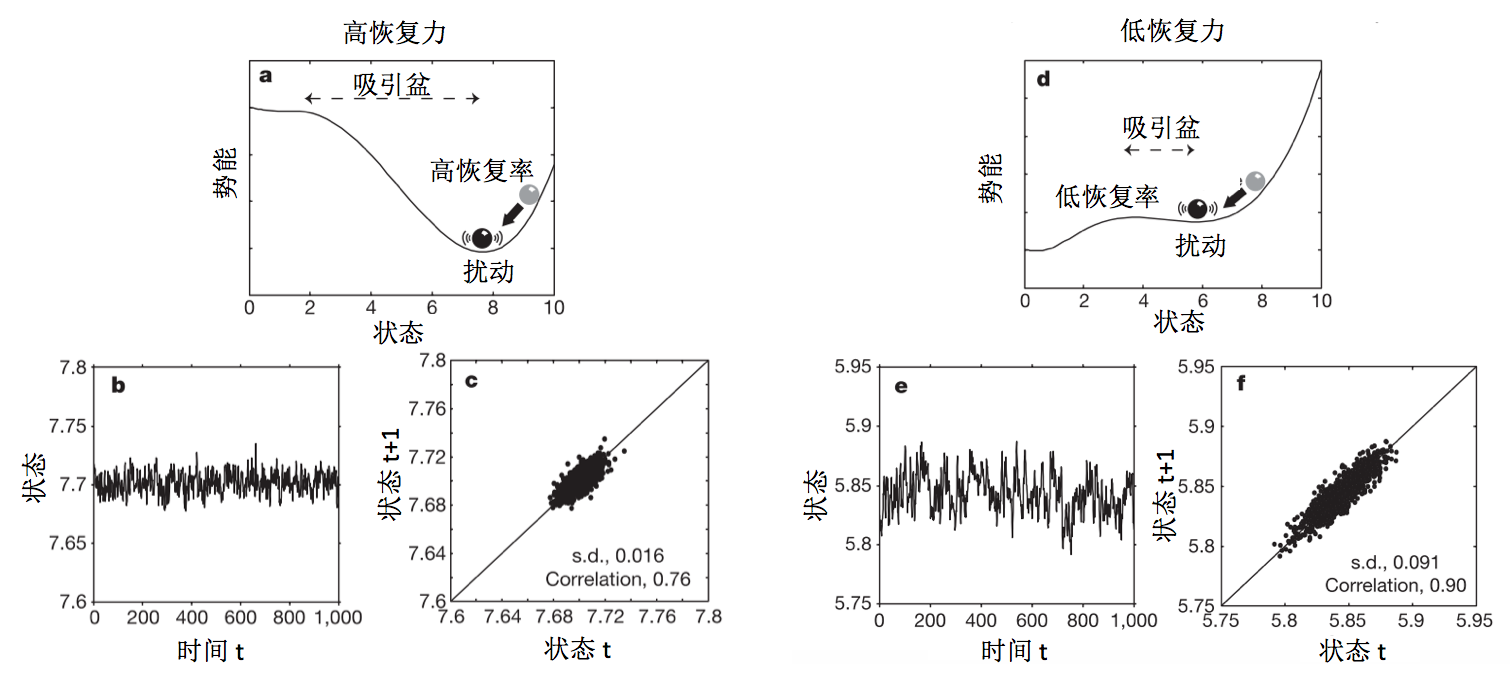
\includegraphics[scale=0.5]{figures/csd-early-warning-signal.png}
\caption{系统临近临界相变状态的特征示意图\cite{scheffer2009early}}
\label{fig:csd-early-warning-signal}
\end{figure}

临界相变点存在是动态系统固有的非线性和随机性导致的结果\cite{bar1997dynamics,endy2005foundations}。
一方面,以上针对预测临界相变点的早期预警特征均以系统的固有随机波动信号,即系统的随机不确定性,为基础。随机不确定性是随机动力学的显著特性\cite{scheffer2001catastrophic},并且“复杂系统理论适用于研究随机动力学系统的临界相变分析”这一论断已得到了大量研究证实\cite{van2007slow,longtin2010stochastic,carpenter2011early}。
另一方面,虽然工业系统似乎与生态系统有所不同,但类似于喷气发动机,机车和轴承这样的工程系统都属于动态系统,并且在复杂的内部因素和环境因素相互作用下表现出非线性行为和随机波动性\cite{strogatz2018nonlinear,cotilla2012predicting}。再者,工业系统的基础是物理学系统\cite{lee2015cyber},物理学系统由于受到外部干扰,例如温度、气候和人为操作等不确定性噪声的影响可增加系统的随机性,以及系统自身的计算复杂性和制造误差,使其普遍存在随机不确定性\cite{wolfram1985origins}。

综上所述,本文认为基于复杂系统随机不确定性分析预测临界相变点的理论可支持本文针对工业系统的失效分析,进而为工业系统的失效机理和普适性{\heiti 早期预警特征}学习提供新思路。再者,此过程只需依赖少量失效敏感时间序列进行学习,可有效应对故障数据小样本、不完备特性的挑战。

%中挖掘出来并且可以为预测潜在自然灾难提供解决方案\cite{scheffer2012anticipating}


% 结构特征
(2)复杂系统临界相变的结构特征

如图\ref{fig:csd-early-warning-structure},复杂系统的结构特征可分为两种,即复杂系统模块间的异构性和复杂系统模块间联系的同构性。其中异构性特征适用于各局部之间相关性不强的系统,而同构性特征适用于各局部之间存在强关联的系统。基于结构特征的改变可对系统临界相变进行预测。分析过程中,可将复杂系统抽象成由各局部构成的复杂网络,每个节点都存在多态性并且与相邻节点有着相互作用关系,比如生态系统中的共生关系、捕猎关系等。若系统中有局部节点发生状态变迁,这样的改变将会传递给相邻节点,以此递归极有可能产生大范围的级联反应,类似于多米诺骨牌效应,最终导致复杂系统整体结构产生变化。2016年,Gao 等人在《Nature》上发表的文章,基于生态系统物种间的关联关系构建相关性结构特征,对系统的变迁进行了很好的预测\cite{gao2016universal}。理论上来说这样的结构特征普遍存在于具有复杂耦合关系的系统中。
\begin{figure}[H]
\centering
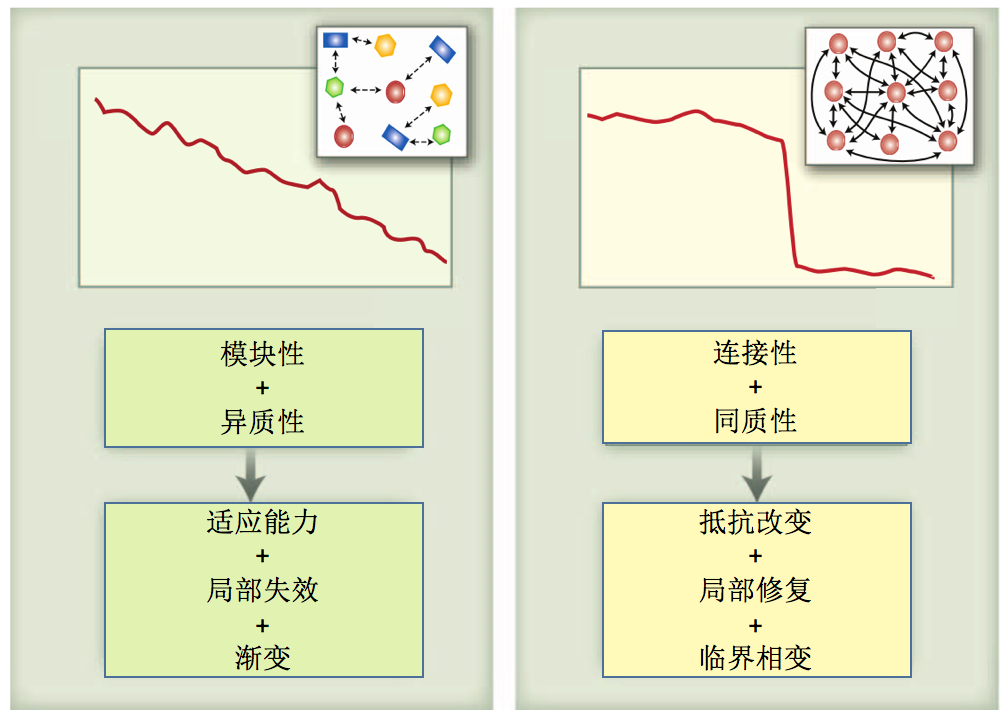
\includegraphics[scale=0.5]{figures/csd-early-warning-structure.png}
\caption{系统临近临界相变点的结构特征\cite{scheffer2012anticipating}}
\label{fig:csd-early-warning-structure}
\end{figure}

在工业系统中,各部件之间或多或少存在相互影响,如何从传感器采集的时序数据中构建相关性结构不变式已经得到广泛关注与研究。在2006年,Jiang 等人通过抽象时序数据之间的关联关系,构建了系统正常状态下的网络结构不变式,当系统局部失效时,结构不变性将会失效,基于此可预测系统异常或故障\cite{jiang2006discovering}。2015年,Han 等人通过构建复杂物理系统的相关性结构特征,对系统级的状态变迁进行了很好的识别\cite{han2015time}。

基于广泛调研与实际观察发现,复杂工业系统各局部的运行机制以及趋势往往存在较大差异,而其与自身历史以及与其他部件间的关联关系可以在给定状态下保持一致,或在可允许范围内轻微波动。综上所述,复杂系统结构特征可以作为{\heiti 高维多模态物理信号建模}的基础,进而有效的支持系统级的健康分析。

\section{生成式对抗网络}
\label{sec:gan-review}

% 深度学习的强大,但
神经网络在特征学习方面取得突破进展\cite{lecun2015deep},比如以绝对优势赢得2012年ImageNet图片分类比赛的深度卷积神经网络AlexNet\cite{krizhevsky2012imagenet}。其他对专家知识依赖很强的领域,比如生物\cite{webb2018deep}、医疗\cite{mirowski2008comparing}、工业\cite{tsui2015prognostics}等领域也纷纷引入神经网络探寻突破,其中,2008年,Mirowski 等人将卷积神经网络与传统机器学习方法逻辑斯蒂回归和支持向量机作比较,基于颅内脑电图扫描器采集的信号来预测癫痫发作,实验结果为:卷积神经网络的误报率最低,基于21个病例进行实验,只有一个误报,而SVM有10个误报\cite{mirowski2008comparing}。

% 大多为判别式模型。存在很多局限,难以进行广泛应用。
以上突破进展大多为基于判别式模型的监督式学习,需要大量标记数据作为训练集,然而获取高质量的标记数据仍是难题。对此,无监督式学习逐渐成为焦点\cite{lecun2015deep}。其中对数据底层分布进行学习的生成式模型是实现无监督式学习的主要方法,目前最主流的生成式模型有全可视信念网络(Fully Visible Belief Network, FVBN)\cite{frey1998graphical}、变分自编码机(Variational AutoEncoder, VAE)\cite{russakovsky2015imagenet}和生成式对抗网络(GAN)\cite{goodfellow2014generative}。GAN 因具有以下优势而倍受青睐:(a) 计算高效:GAN 可以并行生成样本,相比之下FVBN只能串行生成样本效率很低;GAN的训练过程基于快速的反向传播和梯度下降方法,不需要进行马尔可夫链蒙特卡洛(Markov Chain Monte Carlo, MCMC)估计和统计推理(Inference)等耗时的运算,相比之下玻尔兹曼机对MCMC的依赖正面临着计算困难的问题\cite{salakhutdinov2010efficient}。(b) 统计优势:GAN 由生成器和判别器组成,其中生成器负责学习数据的分布,其训练优化由判别器驱动,避免了直接复 制数据的风险,即对过拟合具有天然的抵抗能力。(c)可以学习复杂分布:GAN 由基于神经网络的复杂函数构成,可以学习非常复杂的分布。(d)局限性少:GAN不需要像VAE那样设计变分约束,其基本框架已保证训练过程的全局收敛性;GAN 对生成函数的限制很少,相比之下玻尔兹曼机需要精心设计MCMC过程存在诸多局限。(e)大量实践表明,相比其他主流生成式模型所生成的样本,GAN 生成样本的质量更高。当然GAN也有不足,主要表现为以下两个方面:(a)GAN 的生成器可用于数据生成,但没有显示的表达式。(b)训练过程不稳定,判别器的更新必须要与生成器同步,否则会导致模式崩溃(Mode Collapses),即生成器所表示的分布只能收敛于真实数据集分布的少量模式,缺乏多样性。

GAN 为无监督式学习开辟了新道路,已得到广泛研究和应用,随着不断发展其劣势已逐步得到攻克\cite{radford2015unsupervised},然而鲜有针对时间序列数据的成果,因此本文基于GAN研究{\heiti 通用的无监督式时间序列特征学习}方法具有重要意义。

% 以上优势是我自己根据 tutorial 和 primitive paper 进行总结的结果。

% 来自goodfellow的tutorial
% (1)GAN 可以并行的生成样本,相比于FVBN串行生成样本的方式更高效;(2)GAN 的生成函数限制很少,相比于对马尔可夫过程具有强依赖的玻尔兹曼机(Boltzmann machines)\cite{salakhutdinov2010efficient}更灵活;(3)GAN 的运算不需要类似于玻尔兹曼机运算时的马尔可夫过程,因此更快更高效;(4)GAN不需要像VAE那样设计变分约束,其基本框架已保证训练过程的全局收敛性;(5)大量实践表明,相比于主流生成式模型所生成的样本,GAN 生成样本的质量更高。

% 无监督式学习旨在基于更容易获取的无标记数据学习具有强泛化能力的模型,限制性玻耳兹曼机(Restricted Boltzmann Machine)\cite{salakhutdinov2010efficient}、自动编码机(Auto-Encoder)\cite{vincent2008extracting}和概率图模型(Probability Graph Model)\cite{lee2009convolutional}等都是实现无监督式学习的重要模型,并且大多为学习数据隐含分布的生成式模型。另外,2014 年 Ian J. Goodfellow 等人创造性的提出生成式对抗网络为无监督式学习开辟了新道路\cite{goodfellow2014generative}。
% 【LeCun认为这是近10年来神经网络领域最重要的突破。】

% 介绍 GAN 的定义
(1)生成式对抗网络简介

图\ref{fig:gan-gan}(左)为生成式对抗网络(GAN)的基本结构,其核心由两个神经网络构成,即生成器(Generator, G)和判别器(Discriminator,D)。生成器负责学习数据的分布,基于输入的噪音 \emph{z} 生成逼真的假样本\emph{X'};判别器负责判断输入数据的真假,从输入数据中识别真实样本\emph{X}。GAN的训练过程是生成器和判别器两者间的博弈,生成器基于判别器的反馈不断优化以生成尽可能逼真的样本为目标;与此同时判别器不断提高自身的判别能力来辨别越来越逼真的假样本。原文以造假币的罪犯(生成器)和警察(判别器)之间的博弈作为类比,造假币的罪犯不断提高自身技能以生成逼真的假币为目标,同时警察不断提升自身侦查力以准确地判别钱币真伪为目标。这样的博弈一值持续直到警察(判别器)无法辨别钱币(样本)真伪为止。假设有服从分布$P_{data}$的真实数据集和服从分布$P_{z}$的噪音\emph{z}作为模型输入,GAN的基本结构和训练过程具体的定义如下:
\begin{figure}[H]
\centering
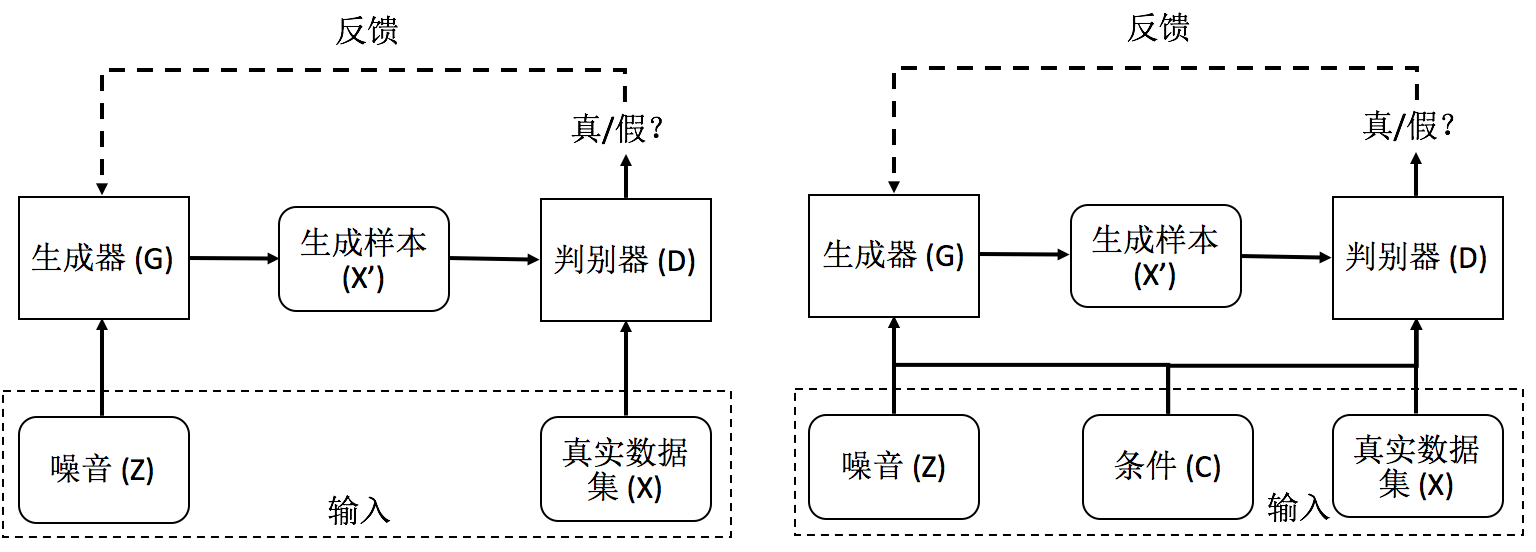
\includegraphics[scale=0.5]{gan-gan.png}
\caption{(左)生成式对抗网络,(右)条件生成式对抗网络}
\label{fig:gan-gan}
\end{figure}

1. 生成器:生成器是以$\theta_{g}$为参数的可导函数,以噪音\emph{z}为先验,通过映射$G(z;\theta_{g})$来学习真实数据分布$P_{data}$,即$G(z;\theta_{g})$实现噪音\emph{z}到样本$x$的映射,并且$G(z;\theta_{g})$可看作分布$P_{g}$表示对$P_{data}$的近似估计。

2. 判别器:判别器是以$\theta_{d}$为参数的可导函数$D(x;\theta_{d})$,对输入样本$x$的真假进行判别(真表示样本$x$来自$P_{data}$,否则表示样本来自$P_{g}$)。判别器实际上是监督式学习中的二分类器,判别器的输出$D(x)$为[0,1]区间上的实数,表示输入样本$x$为真的概率,即表示样本\emph{x}来自$P_{data}$而非$P_{g}$的概率。

3. GAN的训练:GAN的训练过程是由等式\ref{eq:gan-objective-function}定义的最大最小化博弈,该函数基于分类器交叉熵函数来定义,以此为目标函数判别器和生成器通过随机梯度下降和反向传播优化方法进行迭代更新。一方面判别器作为二分类器,以准确判别样本真伪为目标,即最大化真样本的概率并最小化假样本的概率,对应等式\ref{eq:gan-objective-function}的内层最大化过程;另一方面生成器需要基于判别器的反馈进行更新,对应等式\ref{eq:gan-objective-function}外层的最小化过程,即最小化$log(1-D(G(z)))$。等式\ref{eq:gan-objective-function}有全局最优解$P_{g}=P_{data}$,此时判别器无法分辨样本真伪也就不会再产生误差进而训练过程因达到纳什均衡而停止。理论上只要给予GAN足够的能力和训练时间就可达到纳什均衡,具体证明可参考原文\cite{goodfellow2014generative}。
\begin{equation}
\label{eq:gan-objective-function}
  \min_{G}\max_{D} V(D,G) = \mathbb{E}_{x \sim P_{data}(\bf{x})}[log(D(x))] + \mathbb{E}_{z \sim P_{z}(\bf{z})}[log(1-D(G(z)))]
\end{equation}

目标函数\ref{eq:gan-objective-function}便于理论分析,但在实际应用中不总是能产生足够的梯度来优化生成器。在训练初期,生成器的能力很弱,因此其生成的样本质量很差,这样一来判别器很容易辨识生成器生成的假样本,即$D(G(z))$很小,小到接近于0,进而导致$log(1-D(G(z)))$逼近0,以至于梯度消失,此时判别器对生成器只能产生近乎可忽略的微小反馈。因此在实际应用中,对生成器的训练不直接最小化$log(1-D(G(z)))$而是启发性的以最大化$log(D(G(z))$为目标,这样的修改不会影响模型的收敛性并且可以保证生成器在训练初期可得到更大的梯度进行迭代更新。

% % review 当前 GAN 的发展情况
(2)生成式对抗网络研究现状

1. 在结构改进方面

针对GAN训练不稳定的问题,2014年,Mirza 等人提出条件生成式对抗网络(Conditional GAN, CGAN)学习数据的条件概率分布\cite{mirza2014conditional},如图\ref{fig:gan-gan}(右),基于原始GAN加入条件先验(比如样本标记)以限制GAN的训练过程使其不再那么天马行空。在有先验的情况下GAN可以很直接的扩展为CGAN,因此GAN和CGAN通常成对出现。
%值得注意的是,给定的先验条件可以是除样本标记以外的假设或约束。
2015年,Denton 等人基于拉普拉斯算子的金字塔(LAplacian Pyramid)框架融合多个GAN以实现图片数据生成,模型简称为LAPGAN\cite{denton2015deep}。LAPGAN通过若干个基于卷积神经网络的GAN生成多个不同像素的图片,然后融合以上输出结果得到最终的生成样本图片。
2015年,Radford 等人提出深度卷积生成式对抗网络(Deep Convolutional GAN, DCGAN)\cite{radford2015unsupervised},使生成样本的质量有了质的飞跃,此后的大多成果都基于DCGAN进行改进。值得注意的是,虽然LAPGAN也使用卷积神经网络作为基础,但与LAPGAN级联融合不同的是DCGAN改进了生成器中卷积神经网络的基本操作,第一次实现单次生成高分辨率图片。DCGAN几个核心的改进为(a)将判别器的池化层替换为跨步卷积(Strided Convolutions),将生成器的池化层替换为小数跨步卷积(Fractional-Strided Convolutions);(b)生成器和判别器都使用批规范化(Batch Normalization);(c)去掉传统深度神经网络中的全连接隐藏层;(d)对生成器的激活函数作如下设置:除了输出层使用Tanh激活函数以外所有单元都使用ReLU作为激活函数;(e)判别器的所有单元都使用LeakyReLU作为激活函数。

2. 在理论改进方面

有部分研究聚焦于GAN的目标函数和训练方式,尝试对GAN的基础理论进行改进。2016年,Chen 等人提出InfoGAN(Information GAN)实现了完全无监督式学习\cite{chen2016infogan},基于信息论改进GAN的目标函数,通过最大化固定大小的噪音子集和观察样本之间的互信息来鼓励GAN学习可解释且有意义的特征。2017年,Arjovsky 等人提出WGAN(Wasserstein GAN)\cite{arjovsky2017wasserstein},从理论上对GAN的核心困难作出重大改进,主要贡献有:(a)解决了GAN训练不稳定问题;(b)设计瓦瑟斯坦距离(Wasserstein Distances) 作为优化新指标。

3. 在应用探索方面

基于GAN的应用已取得很多重要突破,比如基于GAN实现图片翻译\cite{isola2017image} 、基于GAN实现图片分辨率提升\cite{ledig2016photo} 、基于GAN实现文本到图片的翻译\cite{reed2016generative} 。另外,2016年,Salimans 等人针对GAN的训练问题提出了多种启发式的改进\cite{salimans2016improved},所涉及的方法有特征匹配(Feature matching)、小批量辨识(Minibatch discrimination)、单边标记平滑(One-sided label smoothing)和虚拟批规范化(Virtual batch normalization)。

综上所述,GAN已得到广泛应用和验证。然而现有突破大多局限于计算机视觉和自然语言处理领域,鲜有针对时间序列数据的研究。2018年,Creswell等人为信号处理领域作了有关GAN的研究综述,但鲜有针对时间序列数据的成果\cite{creswell2018generative}。本文至今只关注到医疗领域有相关初探性研究\cite{esteban2017real,yahi2017generative,choi2017generating},然而他们提出的模型都只在一个医疗时间序列数据集上进行验证,不具备普遍适用性。